% Ab hier arabische Seitenzählung und heading Seitenstil
\pagestyle{scrheadings}
\pagenumbering{arabic}

\chapter{Einleitung}


\chapter{Systembeschreibung und Modellierungsansatz}

\section{Demonstratorsytem}
Im Rahmen vorangegangener studentischer Arbeiten ist am Fraunhofer-Institut für Integrierte Schaltungen IIS, Institutsteil Entwicklung Adaptiver Systeme EAS \cite{fraunhoferIISEAS} in Dresden ein Demonstratorsystem entwickelt worden. Langfristig soll dieses Vorteile von Regelungsstrategien auf verteilten Recheneinheiten gegenüber einer zentralen Messgrößenverarbeitung und Stellgrößenberechnung veranschaulichen. Der Demonstrator ist in Abbildung \ref{fig:demonstrator_real} dargestellt.

\begin{figure}[ht]
	\centering
	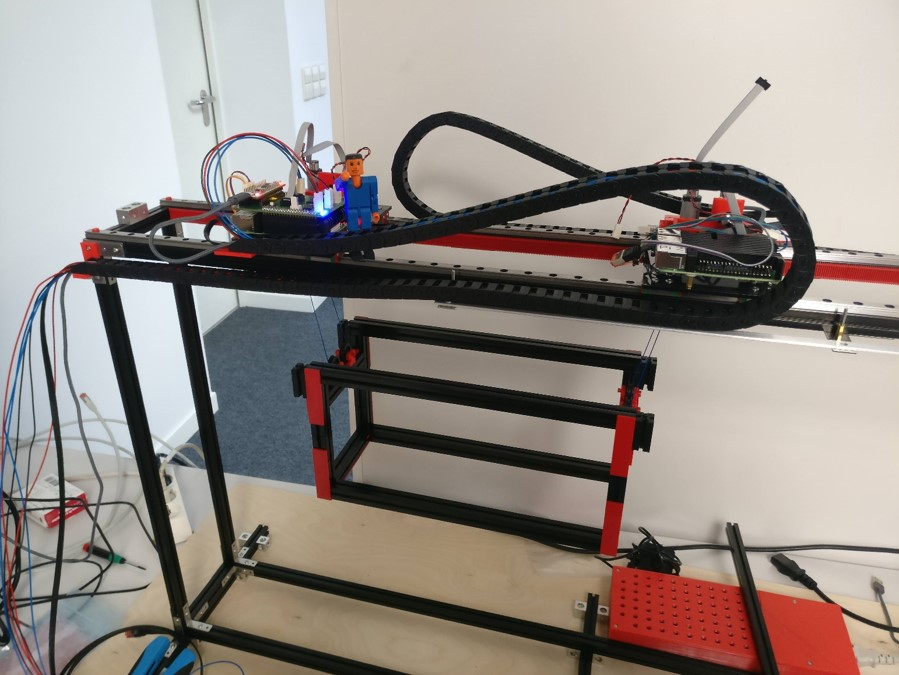
\includegraphics[width=0.75 \textwidth]{Pictures/real_gantry.jpg}
	\caption{Doppelkran-Demonstratorsystem mit Laufkatzen und Last.}
	\label{fig:demonstrator_real}
\end{figure}

Das Demonstratorsystems besteht aus zwei Brückenkränen, die eine gemeinsame Last in einer festen Ebene anheben. Die Kräne befinden sich auf Schienen und verfügen jeweils über einen Raspberry Pi 4B als Hauptrecheneinheit sowie einen STM32-Mikrocontroller für Motoransteuerungen und Messungen. Beide Raspberry Pis können über eine LAN-Verbindung miteinander kommunizieren.

Beide Kräne sind auf Schienen in horizontaler Richtung sowie die Seillängen mit jeweils einem DC-Motor aktuiert. Auf den STM32-Mikrocontroller ist bereits eine eine unterlagerte Strom- beziehungsweise Kraftregelung für diese implementiert.
Messungen der Seillängen und Kranpositionen auf der Schiene erfolgen mittels Inkrementalgebern nach einem anfänglichen Kalibrierungsvorgang. Die Seilwinkel werden mittels mitschwingender Potentiometer bestimmt.




\section{Problembeschreibung und Zielsetzung}
Bei der Bewegung von Containern in Häfen ist ein ruckarmer und gegenüber der Horizontalen stabiler Transport notwendig. Ziel der Studienarbeit ist es deshalb,  bezüglich des vorhandenen Demonstratorsystems eine zentrale Referenzregelstrategie zu entwerfen. Damit soll unter Vorgabe von Sollposen eine Planung von Trajektorien der Last in der Ebene und Folgeregelung zur Überführung dieser zwischen verschiedenen Ruhelagen ermöglicht werden. Diese Überlegungen sollen auf Basis einer Modellierung des Krans als Mehrkörpersystems geschehen. 

\section{Modellierung mittels Lagrange-Formalismus}

\subsection{Lagrange-Gleichungen erster Art}
Die Dynamik mechanischer Systeme lässt sich über Differentialgleichungen, den so genannten Lagrange-Gleichungen beschreiben. Dabei wird eine Menge aus $n$ auftretenden und zeitlich veränderlichen Koordinaten als Konfigurationskoordinaten oder Systemgrößen $\pmb{\theta} = (\theta_1, ..., \theta_n)^T$ bezeichnet. Die zeitlichen Änderungsraten dieser sind die (Konfigurations-)Geschwindigkeiten $\pmb{\dot{\theta}}$ \cite[S.7]{DissKnoll}. 

Die kinetische Energie eines Systems wird im Folgenden durch die Funktion $T$ sowie die potentielle Energie durch $V$ beschrieben. Eine Lagrange-Funktion kann damit folgendermaßen definiert werden:
\begin{equation}
	L(\pmb{\theta}, \dot{\pmb{\theta}}) = T(\pmb{\theta}, \pmb{\dot{\theta}}) - V(\pmb{\theta}).
\end{equation}

Mit den Lagrange-Gleichungen erster Art können Probleme mit Zwangsbedingungen und -kräften dargestellt werden:
\begin{equation}
	\diff{}{t}\left(\partiell{L}{\dot{\theta}_i} \right) - \partiell{L}{\theta_i} = \tilde{Q}_i + Q_i, \quad i = 1, ..., n.
\end{equation}

Die sich auf die jeweilige Koordinate $\theta_i$ beziehende Stellkraft $Q_i = f_i - D_i$ entspricht der verallgemeinerten Kraft, welche sich aus äußeren (Stell-)Kräften $f_i$ sowie internen Reibungskräften $D_i$ zusammensetzt \cite[S. 49]{Lagrange}.

Aus den $m$ holonomen Zwangsbedingungen $g_i(\pmb{\theta}) = 0$ folgen die Zwangskräfte $\tilde{Q}_i$ in Richtung der Koordinate $\theta_i$:
\begin{equation}
	\tilde{Q}_i = \sum_{j = 1}^m \lambda_j G_{ji}(\pmb{\theta})
\end{equation}

Dabei werden die Lagrange-Multiplikatoren $\lambda_j$ unter dieser Beziehung genutzt:
\begin{equation}
	\diff{g_j}{t} = \sum_{i = 1}^n G_{ji}(\pmb{\theta}) \dot{\theta}_i = 0 \quad j = 1, ..., m.
\end{equation}

\subsection{Lagrange-Gleichungen zweiter Art}
Eine alternative Herleitung solcher Systemgleichungen sind die Lagrange-Gleichungen zweiter Art. Bei diesen müssen Zwangskräfte nicht explizit bestimmt werden. Die Bewegungsgleichungen können folgendermaßen aus der Lagrange-Funktion abgeleitet werden:
\begin{equation}
	\diff{}{t}\left(\partiell{L}{\dot{\theta}_i} \right) - \partiell{L}{\theta_i} = Q_i, \quad i = 1, ..., n.
\end{equation} 

Eine stark automatisierte Durchführung dieses Formalismus ist unter Nutzung des Python-Pakets \textit{symbtools} \cite{symbtools} möglich.

-> ggf. dazu in Nextcloud/Präsis Folien zu modeltools -> Matrixdarstellung mit M, C, K, B

Zur Bestimmung der generalisierten Kräfte $Q_i$ wird das Prinzip der virtuellen Arbeit hinzugezogen \cite{VirtualWork}:

\begin{equation}
	\delta W = \sum_{k=1}^l \pmb{F_k} \cdot \frac{\partial \pmb{r_k}}{\partial \theta_1} \delta \theta_1 +\ldots + \sum_{k=1}^l \pmb{F_k} \cdot \frac{\partial \pmb{r_k}}{\partial \theta_n} \delta \theta_n.
\end{equation}

Dabei entspricht bei einem System von $l$ (massebehafteten) Teilchen $\pmb{r_k}$ dem Richtungsvektor zum $k$-ten Partikel, $\pmb{F_k}$ der jeweils entlang dieses Richtungsvektoren angewandten Stellkraft, $\delta \pmb{r_{k}}$ der virtuellen Verschiebung und $\delta \pmb{\theta_{i}}$ der virtuellen Verschiebung der Koordinaten.

Die gesamte virtuelle Arbeit des Systems dieser Teilchen kann also ebenso durch
\begin{equation}
\delta W = Q_1 \delta \theta_1 + \ldots + Q_n\delta \theta_n,
\end{equation}
dargestellt werden, wobei sich die generalisierten Kräfte zu
\begin{equation}
Q_i = \sum_{k=1}^l \frac {\partial \pmb{r_k}} {\partial \theta_i} \cdot \mathbf {F}_{k}  ,\quad i=1,\ldots, n 
\end{equation}
ergeben.
\section{Generierung und Berechnung von DAE-Systemen}
Standardform:
	\begin{align}\label{eq:dae_std}
		\pmb{\dot{x}} &= \pmb{f}(\pmb{x}, \pmb{z}, \pmb{u}, t) \\
		\pmb{0} &= \pmb{g}(\pmb{x}, \pmb{z}, \pmb{u}, t)
	\end{align}
mit $\pmb{x}$ Zustand, $\pmb{z}$ algebraischer Variablen (quasi Zustandsgrößen, die in Systemgleichungen nicht differentiell vorkommen), $\pmb{u}$ Systemeingang, $t$ Zeit.

Differenzieller Index: Minimale Anzahl an Differentiation $\frac{d}{dt}$ der algebraischen Gleichungen (AGL) $\pmb{g}$ (Zwangsbedingungen), damit unter Einbeziehung der Differentialgleichung ein explizites Differentialgleichungssystem aus dem DAE-System entsteht. (Vgl. Systementwurf Mechatronischer Systeme S. 139)

Numerische Integration von DAE-Systemen: 
\begin{itemize}
\item mechanische Systeme mit starrer Kopplung als Zwangsbedingungen allgemein von Index 3
\item Lösung über Indexreduktion auf Index 2 -> Integration über implizites Verfahren
\item Lösung über Indexreduktion auf Index 1 -> Integration über explizites Verfahren + AGL-Löser oder implizites Verfahren
\item Lösung über Indexreduktion auf Index 0 -> Integration über explizites oder implizites Verfahren
\item Bestimmung der Anfangswerte der Integration aus gegebenen AGL oder Gleichungen, die sich im Laufe der Indexreduktion ergeben
\end{itemize}

modeltools führt dabei Reduktion von Index 3 System auf Index 1 System durch.
Hier wird als Solver ODASSL verwendet. Dieser ist modifizierte Version des DASSL Solvers zur Lösung überbestimmter (mehr Gleichungen als Variablen, wieso?) Systeme (singulärer) impliziter DGL ($https://jmodelica.org/assimulo/DAE_OVER_ODASSL.html$). Zu DASSL: https:$//www.openmodelica.org/doc/OpenModelicaUsersGuide/latest/solving.html$

Zum weiterem Verständnis von DAEs: $https://reference.wolfram.com/language/tutorial/NDSolveDAE.html$

weitere Punkte zum behandeln:
- Warum konsistenete AW bei DAE wichtig, Funktionsweise von modeltools mit DAE-Systemen ->DAE System(object)->init? (Präsi zu modeltools unter Präsi in nextcloud)
- Stichpunkte wie in modeltools DAEs aufgestellt werden
- Schritte zur Reduktion auf Index 1 System in modeltoos verstehen, warum ist Reduktion wichtig?

\section{Systematische Flachheitsanalyse von MIMO-Systemen}
Paper Fritzsche, Franke, Knoll Systematische Flachheitsanalyse und Algorithmische $Anleitung: https://github.com/klim-/uc_algorithm/blob/master/doc/user_guide.pdf$

Mathematische Beschreibung eines nichtlinearen Systems in impliziter Form:
\begin{equation}\label{eq:flatness_implicit_ode}
	\pmb{0} = \pmb{F}(\pmb{x}, \pmb{\dot{x}}), \ \pmb{x}(t) \in \mathbb{R}^n
\end{equation}

Wobei $\pmb{x}$ nicht dem Zustandsvektor allein sondern allen Systemgrößen, also Zustandskomponenten und Systemeingangsgrößen entspricht.

Das DAE-System besitzt den Systemgrößenvektor $\pmb{y}$ mit
\begin{equation}
	y
	=
	\begin{pmatrix}
		\pmb{x} \\
		\hline
		\pmb{z}
	\end{pmatrix}
	=
	\begin{pmatrix}
		\pmb{\theta} \\
		\pmb{\dot{\theta}} \\
		\hline
		\pmb{\lambda}
	\end{pmatrix}
\end{equation}

Somit wird unter Berücksichtigung der verallgemeinerten Stellkräfte $\pmb{\tau}$ die implizite DGL gebildet:
\begin{equation}
	\pmb{0} = \pmb{F(w, \dot{w})} \text{ mit } \pmb{w} 
	=
	\begin{pmatrix}
		\pmb{y} \\
		\hline
		\pmb{\tau}
	\end{pmatrix}
	= 
	\begin{pmatrix}
		\pmb{\theta} \\
		\pmb{\dot{\theta}} \\
		\pmb{\lambda} \\
		\hline
		\pmb{\tau}
	\end{pmatrix}
\end{equation}

Mechanische Systeme können über folgende Bewegungsgleichungen dargestellt werden ($2019_Knoll_Heedt_Roebenack_Lagrangian_Modeltools.pdf$):
\begin{align}
	\pmb{0} &= \pmb{M}(\pmb{\theta}) \pmb{\ddot{\theta}} + \pmb{C}(\pmb{\theta}, \pmb{\dot{\theta}}) + \pmb{K}(\pmb{\theta}, \pmb{\dot{\theta}}) + \pmb{G}(\pmb{\theta}) \pmb{\lambda} - \pmb{B}(\pmb{\theta}) \pmb{\tau} \\
	\pmb{0} &= \pmb{g}(\pmb{\theta}) 
\end{align}

(für späteres Kapitel der SA!)
Dieses Doppelkransystem mit den Systemgrößen
\begin{align}
	\pmb{w}
	=
	\begin{pmatrix}
		p_1 \ p_2 \ p_3 \ p_4 \ q_1 \ q_2 \ q_3 \ q_4 \ \dot{p}_1 \ \dot{p}_2 \ \dot{p}_3 \ \dot{p}_4 \ \dot{q}_1 \ \dot{q}_2 \ \dot{q}_3 \ \dot{q}_4 \ \lambda_1 \ \lambda_2 \ \lambda_3 \ \tau_1 \ \tau_2 \ \tau_3 \ \tau_4
	\end{pmatrix}^T
\end{align}

So kann das implizite DAE-System aus den Bewegungsgleichungen und diesen definitorischen Gleichungen beschrieben werden:
\begin{equation}
	(\pmb{I_{6 x 6}}, \pmb{0_{6 x 17}}) \pmb{\dot{w}} = (\pmb{0_{6 x 6}}, \pmb{I_{6 x 6}}, \pmb{0_{6 x 11}}) \pmb{w}
\end{equation}

\section{Statische Eingangs-Ausgangs-Linearisierung}
relativer grad ... (Buch von Röbenack) mit Definition 4.80 usw., aber nich Erzeugung von y Ableitungen

\section{Quasistatische Eingangs-Ausgangs-Linearisierung} 

\chapter{Analytische Modellbildung}

Verschiedene Stufen zur Modellierung im Repo:

Einzelkran:
-model single crane -> ODE System zur kollokierten partiellen Linearisierung, Simulation von ODEs
-DAE lift actuated single crane -> Darstellung als DAE-System mit Hubaktuierung, so dass Regelung mittels virtueller Kraft auf Ruhelage, wenn Schneckengetriebe sperrt.

Doppelkran (double crane notebooks, nur LK Aktuierung):
Prinzipielles Problem, dass in kinetischer Energie T für Lagrange alle abgeleiteten p,q vorkommen müssen
- DAE double crane w1 angle -> G2 in kartesischen Koordinaten und absoluter Lastwinkel, so dass für T nur Trägheitsmoment von Last, nicht Seilen nötig, damit alle p, q enthalten
- DAE double crane w1 angle -> 3 relative Winkel, deshalb auch J in Seilen für T

Doppelkran (lift actuated double crane notebooks, vollständige Aktuierung):
Prinzipielles Problem, dass effiziente Berechnung und Hubaktuierung bei Ruhelage und Schwerkraft wirken (Vgl. Einzelkran DAE lift actuated single crane)
- DAE double crane fully actuated -> 3 Winkel als passive Koordinaten, aber ungelöstes Problem des Findens von konsistenten Anfangswerten
- DAE double crane cartesian -> Gelenke als kartesische Koordinaten, 3 ZB in euklidischen Abständen -> keine cos, sin Terme (daher effiziente Simulation), Längen l1, l2 zunächst als feste Parameter und dann später manuell durch weitere Zustände im Modell mod ergänzt, Trick mit diskreten Massen statt homogener Last wie in Notebook erklärt
- weitere Versuche der Beschreibung mit Winkeln durch Probleme bei T (alle pdot) oder seeehr lange Simulationsdauern nicht zielführend

\section{Analytisches Modell Einzelkran}

\section{Analytisches Modell Doppelkran}

\section{Systemidentifikation}
Trägheitsmoment der Last nach %https://de.wikipedia.org/wiki/Tr%C3%A4gheitsmoment#:~:text=Ein%20Quader%2C%20der%20um%20eine%20Achse%20durch%20den%20Mittelpunkt%20rotiert%2C%20die%20parallel%20zu%20seinen%20Kanten%20c%20liegt.
berechnet zu 0.004553475 kg m m

\chapter{Regelungsstrategie}
\section{Anwendung Flachheitsanalyse am Einzelkran}

\section{Anwendung Flachheitsanalyse am Doppelkran}
Herangezogen: ODE Modell des Gantrys aus Lagrange 1 (ODE flatness analysis simulation)
-> relativ überschaubare mod.eqns (5 Gleichungen)
- eqns.jacobian(ttau), um Spalten zu finden, in denen Größe nur 1 mal vorkommt, so dass keine widersprüchlichen Gleichungen für Bestimmung der Größe 
-> eliminiere Gleichung und Größe aus Zeile, bei der solche Größe gefunden:
-- zunächst tau1(tau2) in 1ter(2ter) Spalte und damit 4te(5te) Zeile/Gleichung zu eliminieren
- bei weiteren Größen keine Spalten mehr in jacobimatrix, in denen Größen nur 1 mal vorkommen, außerdem nun Jacobi-Matrix der Dimension 3x2 
-> Ziel: Durch Linearkombination (Multiplikationen von Links) soll Transformation in Form $\left(\begin{matrix}
1 & 0\\
0 & 1\\
0 & 0
\end{matrix}\right)$ gebracht werden
-> Vorgehen: $w_1 \cdot B_1 = \left(\begin{matrix}
I_2 \\
0_{1 \times 2}
\end{matrix}\right)$ 
-> Bildung der Pseudo-Inversen von B1: $B_{1, pinv} = B_1^{L+}$ sowie Links-Orthokomplement (VR aller Zeilen, die orthogonal auf allen Spalten von B) $B_1^{L \perp}$, also $B^T B_1^{L \perp} = 0$
=> $\left(\begin{matrix}
B_1^{L+} 0 \\
B_1^{L \perp}
\end{matrix}\right)
\left(\begin{matrix}
B_{1, 1} \\
B_{1,2}
\end{matrix}\right)
=
\left(\begin{matrix}
I_2 \\
0_{1 \times 2}
\end{matrix}\right)
$
mit der 3x3 Matrix w1 und 2x2 Matrix $B_{1,1}$, 1x2 Matrix $B_{1,2}$
==> $w_1 = \left(\begin{matrix}
B_1^{L+} \\
B_1^{L\perp}
\end{matrix} \right)$, so dass neuer Gleichungssatz eqns2 = w1 * eqns1, daraus analog wie Anfangs tau1,2 und beide Gleichungen eliminierbar
==> in letzter Gleichung (Zeile) kommen q1,2 nur algebraisch vor:
$s_{2} \left(\left(- p_{1} + q_{1} + s_{2} \cos{\left(p_{3} \right)}\right) \left(l_{0} \sin{\left(p_{3} \right)} - p_{1} \sin{\left(p_{3} \right)} + p_{2} \cos{\left(p_{3} \right)} + q_{2} \sin{\left(p_{3} \right)}\right) + \left(- p_{1} \sin{\left(p_{3} \right)} + p_{2} \cos{\left(p_{3} \right)} + q_{1} \sin{\left(p_{3} \right)}\right) \left(l_{0} - p_{1} + q_{2} - s_{2} \cos{\left(p_{3} \right)}\right)\right) \left(l_{1} l_{2} m_{2} \left(g + \ddot{p}_{2}\right) - l_{1} \tau_{4} \left(p_{2} + s_{2} \sin{\left(p_{3} \right)}\right) - l_{2} \tau_{3} \left(p_{2} - s_{2} \sin{\left(p_{3} \right)}\right)\right) + s_{2} \left(l_{1} l_{2} m_{2} \ddot{p}_{1} + l_{1} \tau_{4} \left(l_{0} - p_{1} + q_{2} - s_{2} \cos{\left(p_{3} \right)}\right) + l_{2} \tau_{3} \left(- p_{1} + q_{1} + s_{2} \cos{\left(p_{3} \right)}\right)\right) \left(l_{0} p_{2} \sin{\left(p_{3} \right)} - l_{0} s_{2} \sin^{2}{\left(p_{3} \right)} - 2 p_{1} p_{2} \sin{\left(p_{3} \right)} + 2 p_{2}^{2} \cos{\left(p_{3} \right)} + p_{2} q_{1} \sin{\left(p_{3} \right)} + p_{2} q_{2} \sin{\left(p_{3} \right)} + q_{1} s_{2} \sin^{2}{\left(p_{3} \right)} - q_{2} s_{2} \sin^{2}{\left(p_{3} \right)}\right) + \left(\left(p_{2} - s_{2} \sin{\left(p_{3} \right)}\right) \left(l_{0} - p_{1} + q_{2} - s_{2} \cos{\left(p_{3} \right)}\right) - \left(p_{2} + s_{2} \sin{\left(p_{3} \right)}\right) \left(- p_{1} + q_{1} + s_{2} \cos{\left(p_{3} \right)}\right)\right) \left(J_{2} l_{1} l_{2} \ddot{p}_{3} + l_{1} s_{2} \tau_{4} \left(- l_{0} \sin{\left(p_{3} \right)} + p_{1} \sin{\left(p_{3} \right)} - p_{2} \cos{\left(p_{3} \right)} - q_{2} \sin{\left(p_{3} \right)}\right) + l_{2} s_{2} \tau_{3} \left(- p_{1} \sin{\left(p_{3} \right)} + p_{2} \cos{\left(p_{3} \right)} + q_{1} \sin{\left(p_{3} \right)}\right)\right) = 0$
kurz:
$\kappa_0 + \kappa_{1, 0} q_1+ \kappa_{0,1} q_2 + \kappa_{1, 1} q_1 q_2 = 0$, so dass hieras OBdA q2 sowie die letzte Gleichung eliminiert werden kann. Die verbleibenden Systemgrößen des Flachenausgangs ergeben sich somit zu $\mathbf{y} = (p_1, p_2, p_3, q_1)^T$. Alle anderen Systemgrößen können durch $\mathbf y(\cdot)$ und dessen Ableitungen parametriert werden. Die Zusammenhänge dafür folgen aus den im Vorhinein eliminierten Gleichungen.´ 

\section{Regelung zur Stabilisierung von Ruhelagen}

\section{Trajektorienplanung}

\section{Trajektorienfolgeregelung}

\subsection{Statische Rückführung}
relativer vektorieller relativer Grad $\pmb{r}$ des MIMO-Systems \cite[S. 194]{NLRT_Roebenack}:\\
- Durch Zeitableitungen der jeweiligen Komponente des flachen Ausgangs $y_i$ kann die damit korrespondierende Komponente des relativen Grades $r_i$ bestimmen. Diese entspricht der Ableitungsordnung, bei der das erste mal ein Eingang explizit auftritt.\\
- Hierbei werden die Zeitableitungen des Ausgangs durch Lie-Ableitungen entlang des Vektorfelds der Systemgleichungen $\pmb{\delta} = \pmb{f} + \pmb{g} \pmb{\tau}$ rekursiv erzeugt: 
\begin{equation}
	y_i^{(k)} = L_{\pmb{\delta}} y_i^{(k-1)}
\end{equation}

-In der folgenden Tabelle sind die daraus bestimmten relativen Grade sowie die dabei explizit auftretenden Eingänge aufgelistet.

\begin{table}[htbp]%
	\centering
	\caption{Relative Grade der Ausgänge und explizites Auftreten der Eingänge.}
	\label{tab:relative_degrees}
	\begin{tabular}{c| c c c c} 
		$i$ & 1 & 2 & 3 & 4 \\ 
		\hline
		$r_i$ & 2 & 2 & 2 & 2\\ 
		\hline
		explizities Auftreten von $\tau_j$ bei $y_i^{(r_i)}$ & $\tau_3, \tau_4$ & $\tau_3, \tau_4$ & $\tau_3, \tau_4$ & $\tau_1, \tau_3$ \\ 
	\end{tabular}
\end{table}

Das Fehlen von $\tau_2$ bei allen dieser Ausgangsableitungen bedeutet für die Entkopplungsmatrix $\pmb{\Lambda}$ (auf Section Statische Eingangs-Ausgangs-Linearisierung verweisen) eine Singularität aufgrund der zweiten Nullspalte, denn der einzige von Null verschiedene Eintrag in $\pmb{g_2}$ erfolgt durch $g_{10, 2} = \frac{1}{m_3}$ und die Lie-Ableitungen $L_f y_i = \dot{y}_i$ geben nur die zeitliche Ableitung des flachen Ausgangs $\dot{\pmb{y}} = (\dot{p}_1, \dot{p}_2, \dot{p}_3, \dot{q}_1)^T$ wieder. So folgt für das relevante Produkt $\partiell{L_{\pmb{f}} y_i}{\dot{q}_2} = 0 \ \forall i$. Allgemeiner gilt, dass ein Eingang $\tau_j$ in den Ausgangsableitungen $y_i^{(r_i)}$ genau dann nicht explizit auftritt, also die $j$-te Spalte von $\pmb{\Lambda}$ eine Nullspalte ist, wenn für alle zugehörigen gemischten Lie-Ableitungen $L_{\pmb{g_j}} L_{\pmb{f}}^{r_i-1} y_i = 0$ gilt \cite[S. 201]{NLRT_Roebenack}:
\begin{align}
	\pmb{\Lambda} = 
	\left(\begin{matrix}
		0 & 0 & \frac{p_{1} - q_{1} - s_{2} \cos{\left(p_{3} \right)}}{m_{2} \sqrt{\left(p_{2} - s_{2} \sin{\left(p_{3} \right)}\right)^{2} + \left(- p_{1} + q_{1} + s_{2} \cos{\left(p_{3} \right)}\right)^{2}}} & \frac{- l_{0} + p_{1} - q_{2} + s_{2} \cos{\left(p_{3} \right)}}{m_{2} \sqrt{\left(p_{2} + s_{2} \sin{\left(p_{3} \right)}\right)^{2} + \left(l_{0} - p_{1} + q_{2} - s_{2} \cos{\left(p_{3} \right)}\right)^{2}}}\\
		0 & 0 & \frac{p_{2} - s_{2} \sin{\left(p_{3} \right)}}{m_{2} \sqrt{\left(p_{2} - s_{2} \sin{\left(p_{3} \right)}\right)^{2} + \left(- p_{1} + q_{1} + s_{2} \cos{\left(p_{3} \right)}\right)^{2}}} & \frac{p_{2} + s_{2} \sin{\left(p_{3} \right)}}{m_{2} \sqrt{\left(p_{2} + s_{2} \sin{\left(p_{3} \right)}\right)^{2} + \left(l_{0} - p_{1} + q_{2} - s_{2} \cos{\left(p_{3} \right)}\right)^{2}}}\\
		0 & 0 & \frac{s_{2} \left(p_{1} \sin{\left(p_{3} \right)} - p_{2} \cos{\left(p_{3} \right)} - q_{1} \sin{\left(p_{3} \right)}\right)}{J_{2} \sqrt{\left(p_{2} - s_{2} \sin{\left(p_{3} \right)}\right)^{2} + \left(- p_{1} + q_{1} + s_{2} \cos{\left(p_{3} \right)}\right)^{2}}} & \frac{s_{2} \left(l_{0} \sin{\left(p_{3} \right)} - p_{1} \sin{\left(p_{3} \right)} + p_{2} \cos{\left(p_{3} \right)} + q_{2} \sin{\left(p_{3} \right)}\right)}{J_{2} \sqrt{\left(p_{2} + s_{2} \sin{\left(p_{3} \right)}\right)^{2} + \left(l_{0} - p_{1} + q_{2} - s_{2} \cos{\left(p_{3} \right)}\right)^{2}}}\\
		\frac{1}{m_{1}} & 0 & \frac{- p_{1} + q_{1} + s_{2} \cos{\left(p_{3} \right)}}{m_{1} \sqrt{\left(p_{2} - s_{2} \sin{\left(p_{3} \right)}\right)^{2} + \left(- p_{1} + q_{1} + s_{2} \cos{\left(p_{3} \right)}\right)^{2}}} & 0
	\end{matrix}\right) .
\end{align}

Analog gilt für den alternativen flachen Ausgang $\pmb{y} = (p_1, p_2, p_3, q_2)^T$ aufgrund des Fehlens von $\tau_1$, welches eine erste Nullspalte von $\pmb{\Lambda}$ impliziert.

Daher ist $\pmb{\Lambda}$ in dieser Form nie regulär und $\pmb{r}$ nie wohldefiniert und dieses System nicht statisch eingangs-ausgangs-linearisierbar. 
Stattdessen können zur Regelung Ansätze mit einer dynamischen Erweiterung oder quasistatischen Zustandsrückführung verfolgt werden. 

\subsubsection{Zustandsrückführung aus Fehlerdynamik}
Nach \cite[S. 195]{NLRT_Roebenack} kann eine lineare Fehlerdynamik, in diesem Fall allerdings bezüglich des Trajektorienfolgefehlers $e := y - y_{\text{ref}}$ und nicht eines Festwerts, angesetzt werden:
\begin{equation}
	e^{(n)} + c_{n-1} e^{(n-1)} + ... + c_{1} \dot{e} + c_{0} e = 0 
	\Leftrightarrow y^{(n)} = y_{\text{ref}}^{(n)} - c_{n-1} e^{(n-1)} - ... - c_{1} \dot{e} - c_{0} e .
\end{equation}
Die Koeffizienten $c_i, \ i \in {0, 1, ..., n-1}$ müssen so gewählt werden, dass das charakteristische Polynom dieser Gleichung ausschließlich Polstellen mit negativem Realteil aufweist.

\subsection{Dynamische Erweiterung}
Die Entkopplungsmatrix $\pmb{\Lambda}$ hat eine Nullspalte, weil $\tau_2$ in keine r Ausgangsableitung $y_i^{(r_i)}$ explizit auftritt. Somit gilt $\text{rang} \ \pmb{\Lambda} = k = 3 < m = 4$. \\

Verhindern von frühzeitigem auftreten der 3 Eingangskomponenten $\tau_1$, $\tau_3$, $\tau_4$ in den entsprechenden Ausgangsableitungen. Dafür: \\
- Ergänzung dieser Eingänge um  in diesem Fall jeweils zwei Integratoren, so dass die neuen Eingangskomponenten bei der selben Ableitungsordnung das erste mal explizit auftreten wie $\tau_2$ und Erweiterung der Systemgleichungen um die folgenden DGL:
\begin{align}
	\begin{split}
		\dot{\tau}_1 &=: \alpha_1 \\
		\dot{\tau}_3 &=: \alpha_3 \\
		\dot{\tau}_4 &=: \alpha_4 \\
		\dot{\alpha}_1 &=: \beta_1 \\
		\dot{\alpha}_3 &=: \beta_3 \\
		\dot{\alpha}_4 &=: \beta_4 .
	\end{split}
\end{align}

- Definition des neuen Eingangsvektors unter Einsortierung der zuvor abwesenden Komponente $\tau_2$ zuletzt $\pmb{\tilde{\tau}} = (\beta_1,  \beta_3,  \beta_4, \tau_2)^T$. \\

- Erweiterung des Zustandsvektors auf $\tilde{\pmb{x}} = (\pmb{x}, \tau_1, \tau_3, \tau_4, \alpha_1, \alpha_3, \alpha_4)^T$ \\
- Umsortierung der Nullspalte von $\pmb{\Lambda}$ auf die letzte Position analog zum neuen Eingangsvektor \\
- Herleitung des Ausgangsableitungen über Lie-Ableitungen entlang erweiterter Zustandsgleichungen  $\pmb{\tilde{\delta}} = \pmb{\tilde{f}} + \pmb{\tilde{g}} \pmb{\tilde{\tau}}$ mit
\begin{align}
	\pmb{\tilde{\delta}} =
	\left(\begin{matrix}
		\pmb{\delta} \\
		\alpha_1 \\
		\alpha_3 \\
		\alpha_4 \\
		\beta_1 \\
		\beta_3 \\
		\beta_4 \\	
	\end{matrix}\right), \quad
	\pmb{\tilde{f}} = \pmb{\tilde{\delta}}|_{\pmb{\tilde{\tau}} = 0}, \quad
	\pmb{\tilde{g}} = \partiell{\pmb{\tilde{\delta}}}{\pmb{\tilde{\tau}}}
\end{align}

und diese sollen nach \cite[S. 195]{NLRT_Roebenack} Gleichung 4.157 jeweils auch über:
\begin{equation}
	y_i^{(r_i)} = L_{\pmb{\tilde{f}}}^{r_i} y_i + L_{\pmb{\tilde{g}_1}} L_{\pmb{\tilde{f}}}^{r_i-1} y_i \beta_1 + L_{\pmb{\tilde{g}_2}} L_{\pmb{\tilde{f}}}^{r_i-1} y_i \beta_3 + L_{\pmb{\tilde{g}_3}} L_{\pmb{\tilde{f}}}^{r_i-1} y_i \beta_4 + L_{\pmb{\tilde{g}_4}} L_{\pmb{\tilde{f}}}^{r_i-1} y_i \tau_2 .
\end{equation}
berechnet werden können.\\
- Für dieses modifizierte System folgt somit stets für $r_i = 4 \ \forall i$. \\

Problem:\\
- Pole müssen weiter links Platziert werden für gutes Folgeverhalten bei Anfangsfehlern (wegen der zusätzlichen Integratoren bei den Eingängen ???) \\
- sehr lange Simulationsdauer

\subsubsection{Änderungen der Trajektorienplanung}
- an beiden Rändern für jede Referenztrajektorie jeweils 2 mal mehr stetig diffbar wegen weiterer differenzierender Zustände von $\tau_1$, $\tau_3$, $\tau_4$ notwendig -> Trajektorienordnung erhöht sich jeweils um 4

\subsubsection{Stabilitätsbetrachtung}

\subsection{Quasi-statische Rückführungen}
Ebenso wie die dynamische Erweiterung kann eine quasi-statische Zustandsrückführung bei einem nicht wohldefiniertem relativen vektoriellen Grad im statischen Ansatz \cite[S. 206]{NLRT_Roebenack}.

\begin{table}[htbp]%
	\centering
	\caption{Auftreten der Eingänge $\tau_j$ bei Ordnung $k$ der Ausgangsableitung $y_i$.}
	\label{tab:relative_degrees}
	\begin{tabular}{ c| c c c c } 
		$k$ & $\tau_1$ & $\tau_2$ & $\tau_3$ & $\tau_4$ \\ 
		\hline
		$y_1^{(k)}$ & 4 & 4 & 2 & 2\\ 
		$y_2^{(k)}$ & 4 & 4 & 2 & 2\\
		$y_3^{(k)}$ & 4 & 4 & 2 & 2\\		
		$y_4^{(k)}$ & 2 & >4 & 2 & 4\\
		$(y_5^{(k)} = q_2^{(k)}$ & >4 & 2 & 4 & 2)\\
	\end{tabular}
\end{table}

- Im Folgenden wird der flache Ausgang $\pmb{y} = (y_1, y_2, y_3, y_4)^T = (p_1, p_2, p_3, q_1)^T$ betrachtet. \\
- Zeitliche Ableitungen werden durch Lie-Ableitungen bezüglich des erweiterten Zustandsvektors $\pmb{\tilde{x}} = (\pmb{x}, \pmb{\tau}, \pmb{\dot{\tau}})^T$ entlang des Vektorfelds der Zustandsgleichungen $\pmb{\tilde{\delta}} = \pmb{\tilde{f}} + \pmb{\tilde{g}} \pmb{\tilde{\tau}}$ mit
\begin{align}
\pmb{\tilde{\delta}} =
\left(\begin{matrix}
\pmb{f} + \pmb{g} \pmb{\tau}\\
\dot{\pmb{\tau}} \\
\ddot{\pmb{\tau}}
\end{matrix}\right)
\end{align}

- $\tau_3$ tritt das erste mal bei $r_1 = 2$ in $\ddot{y}_1$ sowie auch in allen anderen zweiten Ableitungen des flachen Ausgangs auf. Dies gilt nicht für alle weiteren Eingänge, da der relative vektorielle Grad für $r_i = 2 \ \forall i$ nicht wohldefiniert ist. \\
- Außerdem tritt $\tau_4$ auch bei $r_3 = 2$ in $\ddot{y}_1$, $\ddot{y}_2$ und $\ddot{y}_3$, nicht aber in $\ddot{y}_4$ auf. \\
-> Widerspruch zu \cite[S. 206]{NLRT_Roebenack}, bei dem für Auftreten von  $u_2$ der Ausgang $y_2$ noch weiter differenziert werden muss! \\ 
- $\tau_2$ tritt erst bei $r_2 = 4$ in $y_1^{(4)}$, $y_2^{(4)}$ oder $y_3^{(4)}$ auf. \\
- $\tau_1$ tritt erst bei $r_4 = 2$ in $\ddot{y}_4$ auf. \\
- Definition neuer Eingänge:
\begin{align}
\begin{split}
	\ddot{y}_1 = \ddot{p}_1 &=: v_1 = \gamma_1(x, \tau_3, \tau_4) \\
	y_2^{(4)} = p_2^{(4)} &=: v_2 = \gamma_2(x, \tau_1, \tau_2, \tau_3, \tau_4, \dot{\tau}_3, \dot{\tau}_4, \ddot{\tau}_3, \ddot{\tau}_4) \\
	\ddot{y}_3 = \ddot{p}_3 &=: v_3 = \gamma_3(x, \tau_3, \tau_4) \\
	\ddot{y}_4 = \ddot{q}_1 &=: v_4 = \gamma_4(x, \tau_1, \tau_3) .
\end{split}
\end{align}

- Daraus ersichtlich, dass aus einem Gleichungssystem aus $v_1$, $v_3$ und $v_4$ in denen alle Eingänge jeweils affin auftreten, eine explizite Darstellung von $\tau_1$, $\tau_3$ und $\tau_4$ möglich ist. \\
-> im Gegensatz zu \cite[S. 207]{NLRT_Roebenack}, bei dem relative Grade der Ausgangskomponenten aufsteigend sind, so dass kein Gleichungssystem gelöst werden muss, sondern sukzessives Einsetzen vorher berechneter Eingänge und Umstellen der abgeleiteten Ausgänge genügt.\\
- Die Berechnung von $\tau_2$ erfordert größeren Aufwand. Dabei Substitution bisheriger Eingangskomponenten und deren Ableitungen, welche aus Lie-Ableitung entlang von $\pmb{\tilde{\delta}}$ generiert werden. Es folgt ein sehr umfangreicher Ausdruck für $\tau_2$, der bereits zu diesem Zeitpunkt mehr als einhunderttausend Rechenoperationen enthält. \\
- Nach \cite[S. 208]{NLRT_Roebenack} kann eine lineare Fehlerdynamik $\pmb{v}$ entsprechend jeweiligem relativen Grad der Ausgangskomponente angesetzt werden. Für $v_1$, $v_3$ und $v_4$ diese jeweils nur von Zustandskomponenten abhängig, bei $v_2$ allerdings auch von $\ddot{y}_2 = \ddot{p}_2$ und $y_2^{(3)} = p_2^{(3)}$ :
\begin{align}
	\begin{split}
		\ddot{p}_2 &= L_{\pmb{\tilde{\delta}}} \dot{y}_2 = L_{\pmb{\tilde{\delta}}} \dot{p}_2 \\
		p_2^{(3)} &= L_{\pmb{\tilde{\delta}}} \ddot{p}_2.
	\end{split}
\end{align}

und Ableitungen der anderen Komponenten von $\pmb{v}$, die wie folgt berechnet werden:
\begin{align}
	\begin{split}
	    \ddot{e} + c_1 \dot{e} + c_0 e &= 0 \\
		e^{(3)} + c_1 \ddot{e} + c_0 \dot{e} &= 0 \\
		e^{(3)} + c_1 (-c_1 \dot{e} - c_0 e) + c_0 \dot{e} &= 0 \\
		e^{(3)} - c_1^2 \dot{e} + c_0 \dot{e} - c_0 c_1 e &= 0 \\
		e^{(3)} + (c_0 - c_1^2) \dot{e} - c_0 c_1 e &= 0 \\
		e^{(4)} + (c_0 - c_1^2) \ddot{e} - c_0 c_1 \dot{e} &= 0 \\
		e^{(4)} + (c_0 - c_1^2) (-c_1 \dot{e} - c_0 e) - c_0 c_1 \dot{e} &= 0 \\
		e^{(4)} + (c_1^2 - 2 c_0 c_1) \dot{e} + (c_0 c_1^2 - c_0^2) e &= 0 \\
		\Rightarrow \text{ für } i = 1,3,4: \dot{v}_i = y_i^{(3)} &= y_{i, \text{ref}}^{(3)} - (c_{i, 0} - c_{i, 1}^2) \dot{e} + c_{i, 0} c_{i, 1} e \\
		\ddot{v}_i = y_i^{(4)} &= y_{i, \text{ref}}^{(4)} - (c_{i, 1}^3 - 2 c_{i, 0} c_{i, 1}) \dot{e} - (c_{i, 0} c_{i, 1}^2 - c_{i, 0}^2) e,
	\end{split}
\end{align}

so dass sich der neue Eingang $v_2$ wie folgt ergibt:
\begin{equation}
	v_2 = y_2^{(4)} = y_{\text{ref}}^{(4)} - c_{2, 3} (y^{(3)} - y_{\text{ref}}^{(3)}) - c_{2, 2} (\ddot{y} - \ddot{y}_{\text{ref}}) - c_{2, 1} (\dot{y} - \dot{y}_{\text{ref}}) - c_{2, 0} (y - y_{\text{ref}})
\end{equation} 

- Problem mit Singularitäten wenn in den Berechneten Stellgrößen wirklich alle gemessenen Zustandskomponenten $\pmb{x}$ vorkommen statt nur die von $\pmb{y}$ und seinen Ableitungen.

\subsection{Exact feedforward linearization}
An der Stelle einer Kompensation der Nichtlinearität mittels Rückführung der gemessenen beziehungsweise simulierten Zustandskomponenten wie bei der exakten Eingangs-Ausgangs-Linearisierung wird im Folgenden die Referenztrajektorie eingesetzt. \cite{Hagenmeyer2003}

Heuristisch wird eine Fehlerdynamik der Ordnung zwei für alle Komponenten des Koordinatenvektors angesetzt:
\begin{equation}
	\ddot{\pmb{\theta}} = \ddot{\pmb{\theta}}_{\text{ref}} - \pmb{c}_1^T \dot{\pmb{e}} - \pmb{c}_0^T \pmb{e}.
\end{equation}

Aus der Zusammensetzung des Zustandsvektors $\pmb{x} = (\pmb{\theta}, \dot{\pmb{\theta}})^T$ und der eingangsaffine Zustandsraumdarstellung kann außerdem der Zusammenhang:
\begin{equation}
	\ddot{\pmb{\theta}} = \pmb{f}_{[6, 10]}(\pmb{\theta}) + \pmb{g}_{[6, 10]}(\pmb{\theta}) \pmb{\tau}
\end{equation}

hergestellte werden. Dabei bedeutet die Indizierung $\bullet_{[i, j]}$, die Auswahl der Zeilen $i$ bis $j$ von $\bullet$. Da $\pmb{\tau} \in \mathbb{R}^4$ und $\pmb{g}_{[6, 10]} \in \mathbb{R}^{5 \times 4}$ gilt, kann dieser Zusammenhang über die Bildung einer Pseudo-Inversen von $\pmb{g}_{[6, 10]}^+$ nach dem Eingangsvektor aufgelöst werden:
\begin{equation}
	\pmb{\tau}= \pmb{g}^{+}_{[6, 10]} (\pmb{\theta}) \ (\ddot{\pmb{\theta}}_{\text{ref}} - \pmb{c}_{1} \pmb{\dot{e}} - \pmb{c}_{0} \pmb{e} - \pmb{f}_{[6, 10]}(\pmb{\theta})).
\end{equation} 

Unter Einsetzen von $\pmb{\theta}_{\text{ref}}$ in $\pmb{g}_{[6, 10]}^+$ und $\pmb{f}_{[6, 10]}(\pmb{\theta}$ wird die Exact feedforward linearization realisiert:
\begin{equation}
\pmb{\tau}= \pmb{g}^{+}_{[6, 10]} (\pmb{\theta}_{\text{ref}}) \ (\ddot{\pmb{\theta}}_{\text{ref}} - \pmb{c}_{1} \pmb{\dot{e}} - \pmb{c}_{0} \pmb{e} - \pmb{f}_{[6, 10]}(\pmb{\theta}_{\text{ref}})).
\end{equation} 

\subsubsection{Vereinfachung mittels Ausgangsselektion}
Statt der Nutzung einer Pseudo-Inversen kann auch eine Selektion von vier der fünf Gleichungen der Beschleunigungen $\dot{\pmb{\theta}}$ vorgenommen werden. Symbolisch werde dies über eine Selektionsmatrix $S$ dargestellt:
\begin{equation}
	\pmb{S} \ddot{\pmb{\theta}} = \pmb{S}(\ddot{\pmb{\theta}}_{\text{ref}} - \pmb{c}_1^T \dot{\pmb{e}} - \pmb{c}_0^T \pmb{e}) = \pmb{S} \pmb{f}_{[6, 10]}(\pmb{\theta}) + \pmb{S} \pmb{g}_{[6, 10]}(\pmb{\theta}) \pmb{\tau}.
\end{equation} 

Durch die Wahl der letzten 4 Gleichungen kann eine direkte Inversion der somit quadratischen Eingangsmatrix $\pmb{g}_{[7, 10]} = \pmb{S} \pmb{g}_{[6, 10]}$ erfolgen:
\begin{equation}
	\pmb{\tau}= \pmb{g}^{-1}_{[7, 10]}(\pmb{\theta}_{\text{ref}}) \ \pmb{S}(\ddot{\pmb{\theta}}_{\text{ref}} - \pmb{c}_{1} \pmb{\dot{e}} - \pmb{c}_{0} \pmb{e} - \pmb{f}_{[6, 10]}(\pmb{\theta}_{\text{ref}})) \text{ mit } 
	\pmb{S} = 
	\begin{pmatrix}
	0 & 1 & 0 & 0 & 0 \\
	0 & 0 & 1 & 0 & 0 \\
	0 & 0 & 0 & 1 & 0 \\
	0 & 0 & 0 & 0 & 1 \\
	\end{pmatrix}.
\end{equation}

Diese Berechnungsvorschrift der Stellgrößen enthält deutlich weniger Operationen als alle zuvor dargestellten Ansätze. Damit eignet sie sich insbesondere für eine spätere Implementierung ein Echtzeitsystemen sowie sehr viel kürzeren Simulationszeiten. Es ergibt sich für Beispieltrajektorien mit Anfangsfehlern ein sehr gutes Folgeverhalten sowie eine stationäre Genauigkeit.

\subsubsection{Stabilitätsbetrachtung}
Ljapunows erste (indirekte) Methode zeigt, dass entlang ausgewählter Trajektorien zu späteren Zeitpunkten der Simulation Eigenwerte mit positiven Realteil vorkommen. Es ist möglich, dass aufgrund des bis dahin abgeklungenen Folgefehlers keine weitere Destabilisierung des Systems stattfindet, sondern eine stationäre Genauigkeit dennoch erreicht wird. Bis zum Ende der Simulationen weisen alle Eigenwerte erneut einen negativen Realteil auf.

\chapter{war schon}
In den folgenden Abschnitten werden einige Erläuterungen zur \LaTeX-Dokumentenklasse \texttt{ArbeitRST.cls} gegeben werden. Diese basiert auf der Klasse \texttt{scrbook} aus dem \KOMAScript-Paket und kann daher mit Hilfe der Methoden aus diesem Paket modifiziert werden. Für nähere Informationen dazu sei auf die KOMA-Script-Anleitung unter \url{http://www.ctan.org/pkg/koma-script} verwiesen. Das Wichtigste in Kürze gibt es auch in einem Cheatsheet unter \url{https://ctan.org/pkg/latex-refsheet}.

Die Vorlage wurde zuletzt am \today~getestet mit der folgenden Version von \KOMAScript: \KOMAScriptVersion 

\textbf{Changelog}
\begin{itemize}
	\item 09.10.2020: Kompatibilität mit neuen \KOMAScript~Versionen hergestellt (scrpage2 $\rightarrow$ scrlayer-scrpage).
	\item 09.07.2019: Umstellung auf biber/biblatex.
\end{itemize}

% ====================================================
\section{Informationen zu schriftlichen Arbeiten am RST}
Informieren Sie sich in der für Sie relevanten Prüfungsordnung über die \emph{Anzahl der geforderten Exemplare} die eingereicht werden müssen. Bitte beachten Sie, dass jedes dieser Exemplar die \emph{Aufgabenstellung} enthalten muss. Lassen Sie diese bitte beim Binden zwischen der Titelseite und der Selbstständigkeitserklärung einfügen. Eines der Exemplare muss dabei das \emph{originale}, vom Vorsitzenden des Prüfungsausschusses und dem verantwortlichen Hochschullehrer unterzeichnete, Dokument enthalten, bei den restlichen genügen Kopien. Bitte beachten Sie, dass die Arbeit \emph{einseitig} ausgedruckt werden muss. Ausschlaggebend für die fristgemäße Einreichung ist die \emph{Bestätigung des Prüfungsamtes}. Informieren Sie sich daher im \emph{Vorfeld} über die Öffnungszeiten am Abgabetag. Sollte das Prüfungsamt geschlossen haben, ist es in der Regel möglich mit den Mitarbeitern eine individuelle Vereinbarung zu treffen.


% ====================================================
\section{Die Titelseite}
Die Titelseite kann über die in Tabelle \ref{tab:titel} angegebenen Befehle angepasst werden.
\begin{table}[htbp]
\caption{Befehle zum Anpassen der Titelseite}
\label{tab:titel}
\begin{tabular}{lp{12cm}}
Befehl & Bedeutung\\
\toprule
\verb|\author| & legt den Namen des Autors der Arbeit fest\\
\verb|\geburtsdatum| & legt das Geburtsdatum des Autors fest\\
\verb|\geburtsort| & legt das Geburtsort des Autors fest\\
\verb|\title| & legt den Titel der Arbeit fest\\
\verb|\subtitle| & legt den Untertitel der Arbeit fest\\
\verb|\betreuer| & fügt einen Betreuer hinzu\\
\verb|\date| & legt das Einreichungsdatum der Arbeit fest -- \newline wird dieser Befehl nicht aufgerufen wird standardmäßig das zum Kompilationszeitpunkt eingestellte Systemdatum verwendet.\\
\bottomrule
\end{tabular}
\end{table}



% ====================================================
\section{Die ständigkeitserklärung}
In der Selbstständigkeitserklärung werden automatisch der Typ der Arbeit, ihr Titel sowie der Name des Autors übernommen. Der Ort kann über den Befehl \verb|\selbstort| geändert werden, wobei standardmäßig "`Dresden"' verwendet wird. Das Datum ist standardmäßig identisch zum Einreichungsdatum, kann aber mit dem Befehl \verb|\selbstdatum| geändert werden.



% ====================================================
\section{Kurzfassung}
Eine Kurzfassung der Arbeit kann mit dem Befehl \verb|\kurzfassung{deutsch}{englisch}| eingefügt werden. Das erste Argument entspricht dabei der deutschen, das zweite der englischen Version.



% ====================================================
\section{Auswahl des Typs der Arbeit}
Zur Auswahl des Typs der Arbeit steht die Klassenoption \texttt{arbeit} zur Verfügung. Mit dieser können sie zwischen Diplom-, Master- und Studienarbeit sowie dem Bericht zum Forschungspraktikum auswählen:
\begin{table}[hbtp]%
\caption{Auswahl des Typs der Arbeit mittels Klassenoptionen}
\centering
\begin{tabular}{cc}
Diplomarbeit & \verb|\documentclass[arbeit=diplom]{ArbeitRST}|\\
Masterarbeit & \verb|\documentclass[arbeit=master]{ArbeitRST}|\\
Studienarbeit & \verb|\documentclass[arbeit=studie]{ArbeitRST}|\\
Bericht zum Forschungspraktikum & \verb|\documentclass[arbeit=forsch]{ArbeitRST}|
\end{tabular}
\label{}
\end{table}



% ====================================================
\section{Eingebundene Pakete}
In der Dokumentenklasse werden bereits einige \LaTeX-Pakete geladenen. Davon sind die zum Verfassen einer Arbeit möglicherweise relevanten in der Tabelle \ref{tab:pakete} aufgeführt. 
\begin{table}[htbp]%
\centering
\caption{Auswahl eingebundener Pakete}
\label{tab:pakete}
\begin{tabular}{p{3.6cm}p{11.4cm}}
amsmath, amssymb, \newline amsfonts, amsthm & Pakete zum Satz mathematischer Formeln, Dokumentation finden sie unter \newline\url{http://www.ams.org/publications/authors/tex/amslatex},\newline besonders empfehlenswert ist der "`Short Math Guide for \LaTeX"'\\
booktabs & ermöglicht das Setzen "`schöner"' Tabellen, Dokumentation unter \url{http://ctan.org/pkg/booktabs}\\
cite & verbessert einige Aspekte des Zitierens, Dokumentation unter \newline\url{http://ctan.org/pkg/cite}\\
caption, subcaption & Pakete zum Anpassen der Unter- und Überschriften von Tabellen, Grafiken etc., Dokumentation unter \newline\url{http://ctan.org/pkg/caption} \newline\url{http://ctan.org/pkg/subcaption}
\end{tabular}
\end{table}\\
Neben diesen Paketen wird das Paket \verb|hyperref| (\url{http://ctan.org/pkg/hyperref}) zur farbigen Hervorhebung von Verweisen, Links etc.\ eingebunden. Bitte deaktivieren Sie diese Markierungen vor dem Ausdrucken mit Hilfe des Befehls
\begin{center}
\verb|\hypersetup{hidelinks}|.
\end{center}



% ====================================================
\section{Zusätzliche Makros}
In die Dokumentenklasse \texttt{ArbeitRST} wurden einige Makros aufgenommen, die sich bei der Arbeit mit \LaTeX{} als nützlich erwiesen haben.
\begin{table}[htbp]
\centering
\caption{Zusätzliche Makros und Umgebungen}
\begin{tabular}{ccp{9cm}}
Syntax & Ausgabe & Beschreibung\\
\toprule
\texttt{\textbackslash vect\{a\}} & $\vect{a}$ & Umschaltung auf fette Schriftart im Mathemodus-- oft für Vektoren genutzt\\[2ex]
\texttt{\textbackslash diag(a,\textbackslash ldots,z)} & $\diag(a,\ldots,z)$ & Nützlich zur Definition von Diagonalmatrizen\\[2ex]
\texttt{\textbackslash diff[n]\{q\}\{t\}} & $\diff[n]{q}{t}$ & Ableitungen darstellen\\[2ex]
\texttt{\textbackslash partiell[n]\{q\}\{t\}} & $\partiell[n]{q}{t}$ & partielle Ableitungen darstellen\\[2ex]
\texttt{\textbackslash dr} &$\dr$ &Aufrechtes d für Integrale ($\int f(t) \dr t$)\\[2ex]
\texttt{\textbackslash Reals} & $\Reals$ & Körper der reellen Zahlen\\[2ex]
\texttt{\textbackslash Compl} & $\Compl$ & Körper der komplexen Zahlen\\[2ex]
\texttt{\textbackslash Real(a)} & $\Real(a)$ & Realteil von $a$\\[2ex]
\texttt{\textbackslash Imag(a)} & $\Imag(a)$ & Imaginärteil von $a$\\[2ex]
\texttt{\textbackslash norm\{a\}} & $\norm{a}$ & Norm von $a$\\[2ex]
\texttt{\textbackslash abs\{a\}} & $\abs{a}$ & Betrag von $a$\\[2ex]
\texttt{\textbackslash skalprod\{a\}\{b\}} & $\skalprod{a}{b}$ & Skalarprodukt von $a$ und $b$\\[2ex]
\texttt{\textbackslash grad(a)} & $\grad(a)$ & Gradient von $a$\\[2ex]
\texttt{\textbackslash div(a)} & $\div(a)$ & Divergenz von $a$\\
\bottomrule
\end{tabular}
\end{table}


Neben diesen Makros wurden Umgebungen zum Erzeugen von Definitionen (\verb|definition|), Beispielen (\verb|beispiel|), Lemmata (\verb|lemma|) und Bemerkungen (\verb|bemerkung|) definiert.

\begin{table}[htbp]%
\centering
\caption{Beispiele der vordefinierten Umgebungen}
\begin{tabular}{p{8cm}p{7cm}}
Syntax & Ausgabe\\
\toprule
\begin{verbatim}
\begin{definition}[Beispiel]
Beispiel für eine Definitionsumgebung
\end{definition}
\end{verbatim}
&
\begin{definition}[Beispiel]
Beispiel für eine Definitionsumgebung
\end{definition}
\\
\begin{verbatim}
\begin{beispiel}[Beispiel]
Beispiel für eine Beispielumgebung
\end{beispiel}
\end{verbatim}
&
\begin{beispiel}[Beispiel]
Beispiel für eine Beispielumgebung
\end{beispiel}
\\
\begin{verbatim}
\begin{lemma}[Beispiel]
Beispiel für eine Lemmaumgebung
\end{lemma}
\end{verbatim}
&
\begin{lemma}[Beispiel]
Beispiel für eine Lemmaumgebung
\end{lemma}
\\
\begin{verbatim}
\begin{bemerkung}[Beispiel]
Beispiel für eine Bemerkungsumgebung
\end{bemerkung}
\end{verbatim}
&
\begin{bemerkung}[Beispiel]
Beispiel für eine Bemerkungsumgebung
\end{bemerkung}\\
\bottomrule
\end{tabular}
\end{table}



% ====================================================
\section{Weitere Informationen}
Da \LaTeX\ seine Funktionalität im wesentlichen durch frei verfügbare Pakete erhält, ist es günstig eine Distribution zu installieren, die bereits die wesentlichen Pakete enthält und das Hinzufügen weiterer Pakete vereinfacht. Für Windows existiert beispielsweise MiKTeX (\url{http://miktex.org/}) und für Linux TeX Live (\url{http://www.tug.org/texlive/}). Zum Erstellen von \LaTeX-Dokumenten unter Windows hat sich das Programm TeXnicCenter (\url{http://www.texniccenter.org/}), vor allem in Verbindung mit dem Sumatra PDF-Betrachter (\url{http://blog.kowalczyk.info/software/sumatrapdf}), als sehr nützlich erwiesen. Unter Linux gilt dasselbe für das Programm Kile (\url{http://kile.sourceforge.net/}). Zum Erstellen und Verwalten von Bibtex-Dateien wurden gute Erfahrungen mit JabRef (\url{http://jabref.sourceforge.net/}) gemacht. Es existieren zahlreiche Bücher zum Umgang mit \LaTeX, von denen an dieser Stelle nur \cite{MittelbachGoosens05} aufgeführt wird.


%%% Local Variables:
%%% mode: latex
%%% TeX-master: "ArbeitRST"
%%% End:
